\documentclass[tikz, border=3mm]{standalone}
\usepackage{tikz}
\usetikzlibrary{arrows.meta, decorations.markings, positioning}

\begin{document}
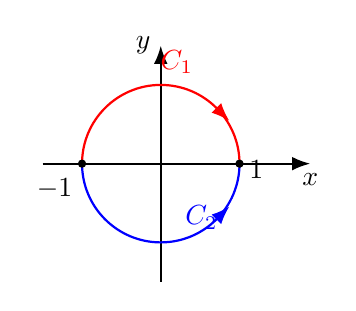
\begin{tikzpicture}[
    >=Latex, % Set default arrow tip style
    axis/.style={->, thick}, % Style for axes
    path/.style={thick}, % Base style for paths
    arrow/.style={decoration={markings, mark=at position #1 with {\arrow{<}}},
     postaction={decorate}}, % Style for arrows on path
    labelstyle/.style={below=2pt}, % Style for -1, 1 labels
    curvelabel/.style={above right=1pt} % Style for C1, C2 labels
]

    % Axes
    \draw[axis] (-1.5, 0) -- (1.9, 0) node[below] {$x$};
    \draw[axis] (0, -1.5) -- (0, 1.5) node[left] {$y$};

    % Define key points and radius
    \coordinate (L) at (-1, 0);
    \coordinate (R) at (1, 0);
    \def\radius{1}

    % Draw Top Arc (C1) - Red, Counter-Clockwise (Right to Left)
    \draw[path, red, arrow=0.25] (R) arc (0:180:\radius) node[curvelabel, red, pos=0.55] {$C_1$};

    % Draw Bottom Arc (C2) - Blue, Clockwise (Right to Left)
    \draw[path, blue, arrow=0.25] (R) arc (360:180:\radius) node[curvelabel, blue, pos=0.45] {$C_2$};

    % Add labels for -1 and 1
    \node[labelstyle, black, below left] at (L) {$-1$};
    \node[labelstyle, black, right] at (R) {$1$};

    % Add dots at intersection points (optional)
    \fill (L) circle (1.5pt);
    \fill (R) circle (1.5pt);

\end{tikzpicture}
\end{document}